공학적 문제에서 만나는 많은 함수혹은 방정식들은 보존 법칙(conservation law)에 기초를 두고 있다. 이와 같은 법칙이 적용되는 양으로는 질량, 에너지 그리고 운동량 등이 있다. 이들 원리들은 수학적 용어를 사용하여 모델링되어지는 양(quantity)의 수준(level) 또는 응답(response)으로 표현되는 시스템의 거동(behavior)을, 시스템의 성질(property) 또는 특성(characteristic)과 외부 자극(stimuli) 또는 시스템에 작용하는 강제함수(forcing function)등에 관련시키는 평형(balance) 또는 연속방정식(continuity equation)을 이끌어내게 된다.
\ref{part1}부에서, 단일요소 시스템은 근-위치 방법들을 사용하여 풀 수 있는 단일 방정식이었다면, 다중요소 시스템은 동시에 연립하여 풀어야 할 상호 연관된 방정식으로 표현된다. 이들 방정식들은 서로 연관되어 상호 작용을 하는데 그 이유는 시스템의 한 부분이 다른 부분에 의하여 영향을 받기 때문이다. 이러한 다중요소 문제들은 집중(lumped) 또는 분산(distributed) 변수의 수학적 모델 모두에서 발생하게 된다.
\begin{figure}[!hbpt]
\centering
\subfigure[구성 요소들이 상호 연관되어 있는 집중 변수시스템(lumped variable system)]{
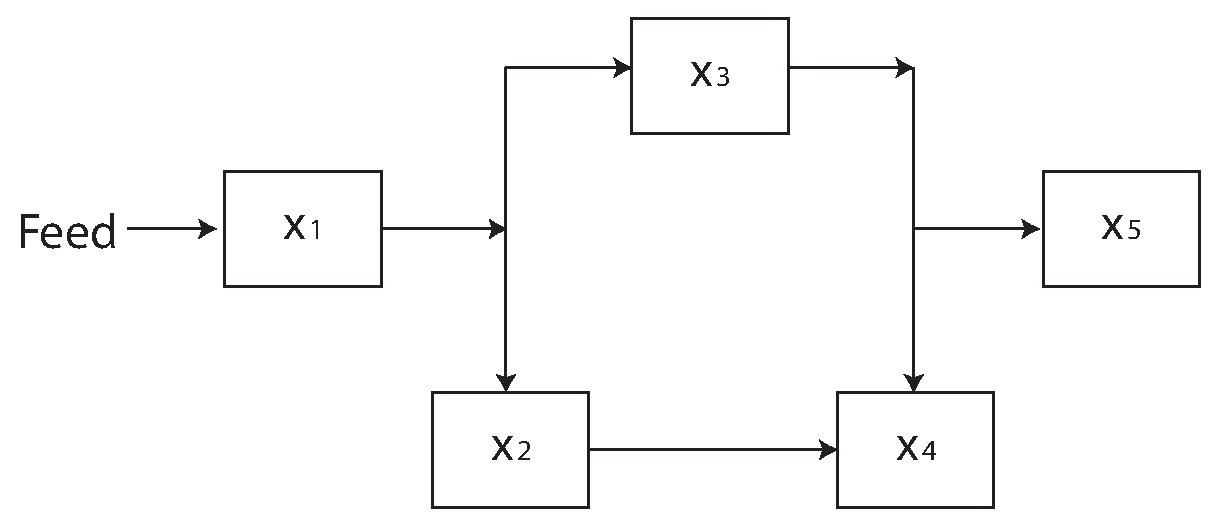
\includegraphics[keepaspectratio=true,width=0.8\linewidth]{figs2/pt3-1a.eps}}
\subfigure[연속체로 이루어진 분산 변수 시스템(distributed variable system]{
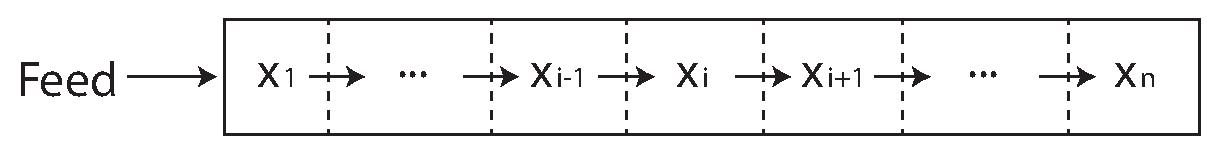
\includegraphics[keepaspectratio=true,width=0.8\linewidth]{figs2/pt3-1b.eps}}
\caption{선형대수 방정식을 사용하여 모델링할 수 있는 두가지 시스템}
\label{fig:pt3-1}
\end{figure}

\section{Gauss 소거법\\(Gauss elimination)}
Gauss 소거법은 연립 방정식의 해를 구하는 최초의 방법 중의 하나이지만, 현재에도 매우 중요한 알고리즘의 하나로 남아 있으며, 널리 알려져 있는 상용소프트웨어 패키지상에서 선형 방정식의 해를 구하는데 기초가 되고 있다.
\subsection{도식적 방법}
좌표의 한 축이 $x_{1}$이고, 다른 축이 $x_{2}$인 직교좌표계상에서 두 방정식을 그래프로 그린 후 그 교점으로부터 해를 얻는다.
\begin{align*}
a_{11}x_{1}+a_{12}x_{2}&=b_{1}\\
a_{21}x_{1}+a_{22}x_{2}&=b_{2}
\end{align*}
두 식을 $x_{2}$항으로 표현하여 기울기와 $x_{2}$ 절편을 얻는다.
\begin{align*}
x_{2}&=-\left(\frac{a_{11}}{a_{12}}\right)x_{1}+\frac{b_{1}}{a_{12}}\\
x_{2}&=-\left(\frac{a_{21}}{a_{22}}\right)x_{1}+\frac{b_{2}}{a_{22}}
\end{align*}
이 직선들을 직교좌표계상에서 $x_{2}$를 세로축, $x_{1}$을 가로축으로 하여 그리면, 두 선들이 만나는 점의 좌표값 $x_{1}$과 $x_{2}$가 해가 된다.
도식적 방법을 사용하여 다음 방정식을 풀면,
\begin{align*}
3x_{1}+2x_{2}&=18\\
-x_{1}+2x_{2}&=2
\end{align*}

\begin{figure}[!hbpt]
\centering
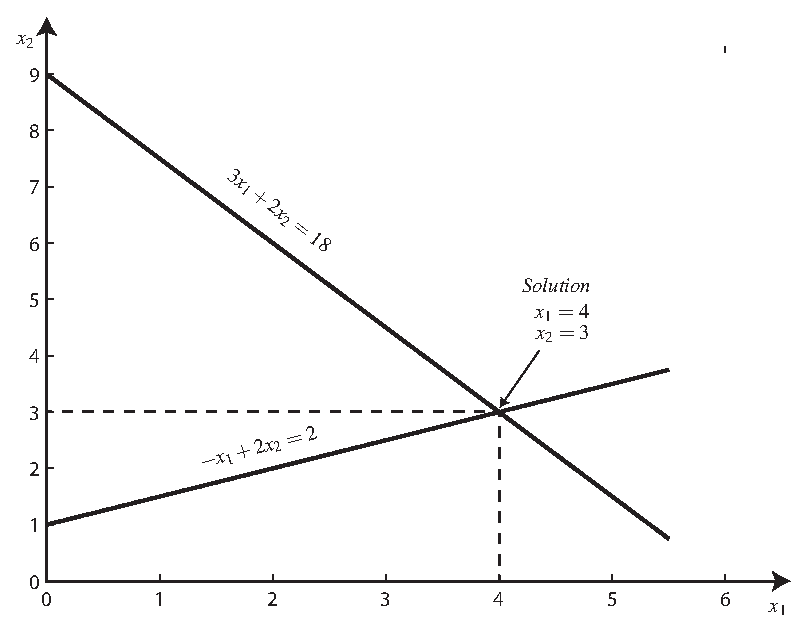
\includegraphics[keepaspectratio=true,width=0.7\linewidth]{figs2/p8_1.eps}
\caption{2개의 연립 선형대수 방정식의 도식적 방법}
\label{fig:8-1}
\end{figure}
Figure~\ref{fig:8-2}는 연립 선형 방정식을 풀 때 발생할 수 있는 세가지 경우를 보여주고 있다. Figure~\ref{fig:8-2a}는 두 개의 직선이 평행한 경우로, 두 직선이 서로 교차하지 않아 해가 존재하지 않는다. Figure~\ref{fig:8-2b}는 두 개의 직선이 일치하는 경우. 이 두 경우의 시스템을 특이(singular)하다고 한다. 특이한 경우에 매우 가까운 시스템인 Figure~\ref{fig:8-2c}의 경우는 시스템에 문제를 발생시킬 수 있는 시스템으로 불량조건(ill-conditioned)을 갖는다고 말한다.
\begin{figure}[!hbpt]
\centering
\subfigure[해가 존재하지 않는 경우]{\label{fig:8-2a}
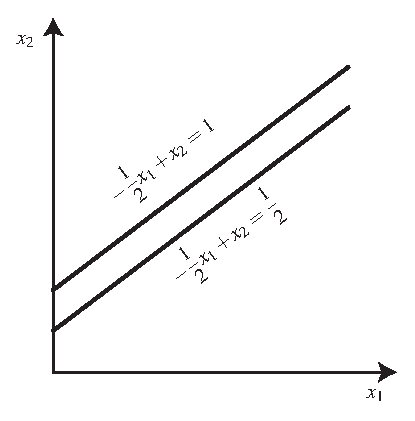
\includegraphics[keepaspectratio=true,width=0.3\linewidth]{figs2/p8_2a.eps}}
\subfigure[해가 무한히 많은 경우]{\label{fig:8-2b}
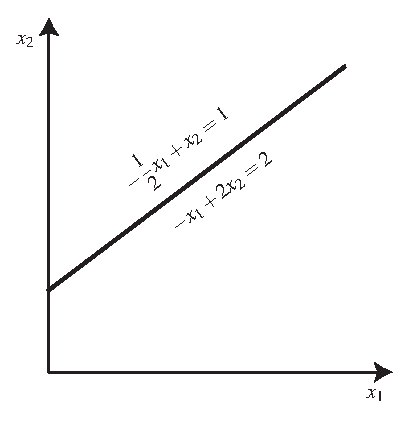
\includegraphics[keepaspectratio=true,width=0.3\linewidth]{figs2/p8_2b.eps}}
\subfigure[불량조건 시스템]{\label{fig:8-2c}
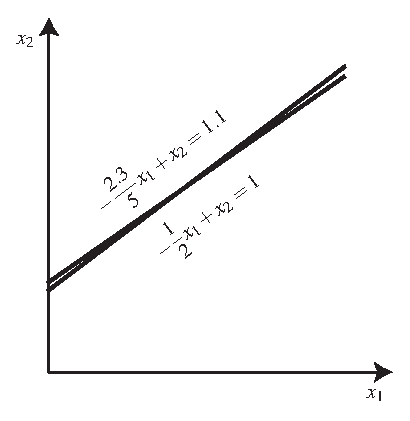
\includegraphics[keepaspectratio=true,width=0.3\linewidth]{figs2/p8_2c.eps}}
\caption{특이하고 불량조건을 갖는 시스템}
\label{fig:8-2}
\end{figure}

\subsection{행렬식과 Cramer 공식}
Cramer 공식(Cramer's rule)은 방정식의 수가 적을 때 매우 적합한 또 다른 해법이다.Cramer 식을 수행하는데 사용될 행렬식(determinant)의 대하여 알아야 한다. 행렬식은 행렬이 불량조건인지의 여부를 판단하는데도 사용된다.
\subsubsection{행렬식}
행렬식을 다음과 같은 세 개의 연립방정식의 경우에 대하여 설명하면,
\begin{equation*}
\mathbf{AX}=\mathbf{B}
\end{equation*}
여기서 $\mathbf{A}$는 계수행렬(coefficient matrix)로써
\begin{equation*}
\mathbf{A}=\begin{bmatrix}a_{11}&a_{12}&a_{13}\\a_{21}&a_{22}&a_{23}\\a_{31}&a_{32}&a_{33}\end{bmatrix}
\end{equation*}
이 시스템의 행렬식 $D$는 다음과 같이 방정식의 계수로부터 얻어진다.
\begin{equation}\label{eq:8-2}
D=\left|\begin{array}{ccc}a_{11}&a_{12}&a_{13}\\a_{21}&a_{22}&a_{23}\\a_{31}&a_{32}&a_{33}\end{array}\right|
\end{equation}
행렬식$D$와 계수행렬$\mathbf{A}$는 같은 요소들로 구성되어 있지만, 완전히 다른 수학적 개념을 가지고 있다. 이 때문에 행렬은 bold 폰트를 사용하여 표시하고 구성요소는 대괄호를 사용하여 나타내지만 , 행렬식은 스칼라값이기 때문에 normal 폰트를 사용하고 구성요소는 절대값 괄호로 표시한다. 2차 행렬식은 다음 식(\ref{eq:8-3})과같이 표현한다.
\begin{align}
D&=\left|\begin{array}{cc}a_{11}&a_{12}\\a_{21}&a_{22}\end{array}\right|\\
&=a_{11}a_{22}-a_{12}a_{21}\label{eq:8-3}
\end{align}
3차 행렬식[식(\ref{eq:8-2})]의 경우, 행렬식의 값은 다음과 같이 계산한다.
\begin{equation}
D=a_{11}\left|\begin{array}{cc}a_{22}&a_{23}\\a_{32}&a_{33}\end{array}\right|-a_{12}\left|\begin{array}{cc}a_{21}&a_{23}\\a_{31}&a_{33}\end{array}\right|+a_{13}\left|\begin{array}{cc}a_{21}&a_{22}\\a_{31}&a_{32}\end{array}\right|
\end{equation}
여기서 $2\times2$의 행렬식을 소행렬식(minor)라고 한다.
\subsubsection{Cramer 공식}
이 공식은 연립 선형대수 방정식에서의 각각의 미지수는 두개의 행렬식의 비로 표시될 수 있다는 것을 말해준다. 다음의 $n\times n$ 연립 선형대수 방정식에서,
\begin{equation*}
\mathbf{AX}=\mathbf{B}
\end{equation*}
$n\times n$크기의 행렬 $\mathbf{A}$의 행렬식이 $0$을 가지지 않는다면, 벡터 $\mathbf{X}=(x_{1},\cdots,x_{n})^T$의 $x_{i}$는 다음 식을 통해 구할 수 있다.
\begin{equation}
x_{i}=\frac{\left|\mathbf{A}_{i}\right|}{\left|\mathbf{A}\right|}
\end{equation}
여기서, $\mathbf{A}_{i}$는 행렬 $A$의 $i$번째 열을 벡터 $\mathbf{B}$로 대체한 행렬이다.
\\
\framebox{예제} \textbf{Cramer 공식}\\
\rule{\textwidth}{0.1pt}
Cramer 공식을 사용하여 다음의 방정식을 풀어라.
\begin{align*}
0.3x_{1}+0.52x_{2}+x_{3}&=-0.01\\
0.5x_{1}+x_{2}+1.9x_{3}&=0.67\\
0.1x_{1}+0.3x_{2}+0.5x_{3}&=-0.44
\end{align*}
\framebox{해} 행렬식 $D$는 다음과 같이 쓸 수 있다.
\begin{equation*}
D=D=\left|\begin{array}{ccc}0.3&0.52&1\\0.5&1&1.9\\0.1&0.3&0.5\end{array}\right|
\end{equation*}
소행렬식을 구하면,
\begin{align*}
D_{1}&=\left|\begin{array}{cc}1&1.9\\0.3&0.5\end{array}\right|=1(0.5)-1.9(0.3)=-0.07\\
D_{2}&=\left|\begin{array}{cc}0.5&1.9\\0.1&0.5\end{array}\right|=0.5(0.5)-1.9(0.1)=0.06\\
D_{3}&=\left|\begin{array}{cc}0.5&1\\0.1&0.3\end{array}\right|=0.5(0.3)-1(0.1)=0.05
\end{align*}
$\mathbf{A}$의 행렬식은
\begin{equation*}
D=0.3(-0.07)-0.52(0.06)+1(0.05)=-0.0022
\end{equation*}
Cramer 공식을 적용하면, 해는 다음과 같이 구할 수 있다.
\begin{align*}
x_{1}&=\frac{\left|\begin{array}{ccc}-0.01&0.52&1\\0.67&1&1.9\\-0.44&0.3&0.5\end{array}\right|}{-0.0022}=\frac{0.03278}{-0.0022}=14.9\\
x_{2}&=\frac{\left|\begin{array}{ccc}0.3&-0.01&1\\0.5&0.67&1.9\\0.1&-0.44&0.5\end{array}\right|}{-0.0022}=\frac{0.0649}{-0.0022}=-29.5\\
x_{3}&=\frac{\left|\begin{array}{ccc}0.3&0.52&-0.01\\0.5&1&0.67\\0.1&0.3&-0.44\end{array}\right|}{-0.0022}=\frac{-0.04356}{-0.0022}=19.8
\end{align*}
\rule{\textwidth}{0.1pt}\\
방정식의 개수가 세 개 이상이 되면, 방정식의 개수가 증가함에 따라 행렬식을 수작업(또는 컴퓨터에 의하여)에 의하여 구하는 데에 매우 많은 시간이 소비되므로, Cramer 공식은 비현실적이라고 할 수 있다.
\subsection{Gauss 소거법}
\begin{wrapfigure}{r}{0.5\textwidth}
\centering
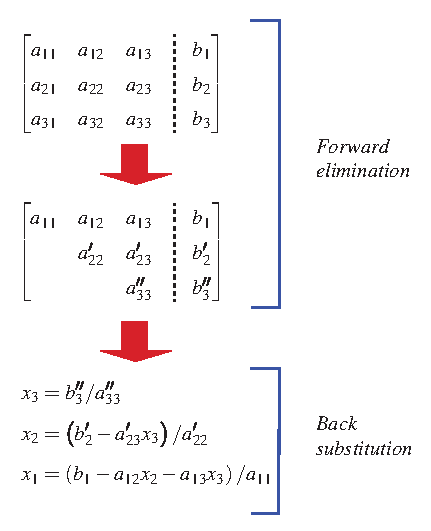
\includegraphics[keepaspectratio=true,width=0.48\textwidth]{figs2/p8-3.eps}
\caption{Gauss 소거법의 두단계}
\label{fig:8-3}
\end{wrapfigure}
Gauss 소거법은 전진소거(forward elimination)와 후진대입(back substitution)의 방법으로 나뉜다. 이 방법은 컴퓨터상에서 구현하기에 이상적이지만, 신뢰성 있는 알고리즘을 위하여 약간의 수정이 필요하다. 특히, 컴퓨터 프로그램에서는 0으로 나누는 경우를 피해야한다. 
다음과 같이 일반적인 $n$개의 방정식을 풀고자 한다.
\begin{align}
a_{11}x_{1}+a_{12}x_{2}+a_{13}x_{3}+\cdots+a_{1n}x_{n}&=b_{1}\label{eq:8-12a}\\
a_{21}x_{1}+a_{22}x_{2}+a_{23}x_{3}+\cdots+a_{2n}x_{n}&=b_{2}\label{eq:8-12b}\\
\vdots\qquad{}&=\vdots\nonumber\\
a_{n1}x_{1}+a_{n2}x_{2}+a_{n3}x_{3}+\cdots+a_{nn}x_{n}&=b_{n}\label{eq:8-12c}
\end{align}
\subsubsection{미지수의 전진소거(forward elimination)}
첫 번째 단계는 연립방정식을 상부삼각(upper triangular) 시스템으로 만드는 것이다. 2번째 $x_{1}$항을 소거하기 위하여 식(\ref{eq:8-12a})에 $a_{21}/a_{11}$을 곱하면,
\clearpage
\begin{equation}\label{eq:8-13}
a_{21}x_{1}+\frac{a_{21}}{a_{11}}a_{12}x_{2}+\frac{a_{21}}{a_{11}}a_{13}x_{3}+\cdots+\frac{a_{21}}{a_{11}}a_{1n}x_{n}=\frac{a_{21}}{a_{11}}b_{1}
\end{equation}
이 방정식을 식(\ref{eq:8-12b})에서 빼면,
\begin{align}
\left(a_{22}-\frac{a_{21}}{a_{11}}a_{12}\right)x_{2}+\cdots+\left(a_{2n}-\frac{a_{21}}{a_{11}}a_{1n}\right)x_{2}&=b_{2}-\frac{a_{21}}{a_{11}}b_{1}\\
a'_{22}x_{2}+\cdots+a'_{2n}x_{n}&=b'_{2}
\end{align}
이러한 방식으로 나머지 방정식에 대해서도 같은 절차를 반복한다. 그 절차를 $n-1$번을 반복수행하면,
\begin{align}
a_{11}x_{1}+a_{12}x_{2}+a_{13}x_{3}+\cdots+a_{1n}x_{n}&=b_{1}\label{eq:8-14a}\\
a'_{22}x_{2}+a'_{23}x_{3}+\cdots+a'_{2n}x_{n}&=b'_{2}\label{eq:8-14b}\\
a'_{32}x_{2}+a'_{33}x_{3}+\cdots+a'_{3n}x_{n}&=b'_{3}\label{eq:8-14c}\\ 
\vdots\qquad{}&=\vdots\nonumber\\
a'_{n2}x_{2}+a'_{n3}x_{3}+\cdots+a'_{nn}x_{n}&=b'_{n}\label{eq:8-14d}
\end{align}
식(\ref{8-12a})를 피벗방정식(pivot equation)이라고 하고, $a_{11}$을 피벗계수(pivot coefficient) 또는 피벗요소(pivot element)라고 한다. 계속해서 식(\ref{eq:8-14b})를 시작으로 나머지 피벗방정식을 아래로 내리면서 소거를 해나갈 수 있다. 이 과정에서 마지막 작업은 $n$번째 방정식으로부터 $x_{n-1}$을 소거하기 위하여 $(n-1)$번째 방정식을 사용하는 것이다. 이 시점에서 시스템은 상부삼각(upper triangular) 시스템으로 변환된다.
\begin{align}
a_{11}x_{1}+a_{12}x_{2}+a_{13}x_{3}+\cdots+a_{1n}x_{n}&=b_{1}\label{eq:8-15a}\\
a'_{22}x_{2}+a'_{23}x_{3}+\cdots+a'_{2n}x_{n}&=b'_{2}\label{eq:8-15b}\\
a''_{33}x_{3}+\cdots+a''_{3n}x_{n}&=b''_{3}\label{eq:8-15c}\\
\ddots\qquad{}&=\vdots\nonumber\\
a_{nn}^{(n-1)}x_{n}&=b_{n}^{(n-1)\label{eq:8-15d}}
\end{align}
\subsubsection{후진대입(back substitution)}
식(\ref{eq:8-15d})는 $x_{n}$값을 얻는데 사용할 수 있다.
\begin{equation}\label{eq:8-16}
x_{n}=\frac{b_{n}^{(n-1)}}{a_{nn}^{(n-1)}}
\end{equation}
이 결과를 $(n-1)$번째 방정식에 대입하여 $x_{n-1}$을 얻게 된다. 나머지 $x$들의 값을 얻기 위하여 반복되는 이 후진대입의 과정은 다음 식과 같다.
\begin{equation}\label{eq:8-17}
x_{i}=\frac{b_{i}^{(i-1)}-\sum\limits_{j=i+1}^{n}a_{ij}^{(i-1)}x_{j}}{a_{ii}^{(i-1)}}\quad\text{for $i=n-1$, $n-2$, $\cdots$, $1$}
\end{equation}

\begin{algorithm}
Let loop $k$ control the elimination step, loop $i$ control $i-$th row accessing and loop $j$ control $j-$th column accessing, the sequential Gaussian Elimination alogithms is decribed as follow(in numerical program, vector $\mathbf{B}$ is stored as $(n+1)-$th column of matrix $\mathbf{A}$):
\begin{algorithmic}
\For{$k=1$ to $n-1$}
  \For{$i=k+1$ to $n$}
    \State $a_{ik}=a_{ik}/a_{kk}$;
    \For{$j=k+1$ to $n+1$}
      \State $a_{ij}=a_{ij}-a_{ik}\times a_{kj}$;
    \EndFor
  \EndFor
\EndFor
\end{algorithmic}
Note that since the entries in the lower triangluar matrix vanish after elimination, their space is used to store multipliers $a_{ik}=a_{ik}/a_{kk}$
\caption{Forward Elimination}
\end{algorithm}

\begin{algorithm}
\begin{algorithmic}
\For{$i=n$ to $1$}
  \For{$j=i+1$ to $n$}
    \State $x_{i}=x_{i}-a_{ij}\times x_{j}$;
  \EndFor
  \State $x_{i}=x_{i}/a_{ii}$;
\EndFor
\end{algorithmic}
Note that $x_{i}$ is stored in the space of $a_{i,n+1}$.
\caption{Backward Substitution}
\end{algorithm}
\subsection{피벗화}
피벗요소가 0인 경우에는 정규화 과정에서 0으로 나누는 경우가 발생하고 0이 아닌경우에도 0에 가까운 피벗일 수록 반올림오차가 생겨날 수 있기 때문에 문제가 발생할 수 있다. 따라서, 각 행들이 정규화되기 전에, 피벗요소 아래에 열중에 가장 큰 계수를 찾은 후, 가장 큰 요소가 피벗요소가 되도록 행의 위치를 교환하여야 한다. 이를 부분피벗화(partial pivoting)라고 한다. 만일 행뿐만 아니라 열에서도 가장 큰 요소를 찾아 위치교환을 한다면, 완전피벗화(complete pivoting)라고 부른다.



%\subsection{Gauss-Jordan법}
%Gauss-Jordan법은 Gauss 소거법의 변형으로 차이점은 피벗요소 밑에 있는 방정식뿐만 아니라 모든 방정식으로 부터 미지수가 소거된다. 또 모든 행을 각각의 피멋요소로 나누어 정규화된다. 따라서 소거단계의 결과로 삼각행렬이 아닌 단위행렬(identity matrix)을 얻게 된다. 결과적으로 이 방법의에서는 해를 구하기 위하여 후진대입을 할 필요가 없다.
%\begin{equation}
%\begin{bmatrix}a_{11}&a_{12}&a_{13}&\vdots&b_{1}\\a_{21}&a_{22}&a_{23}&\vdots&b_{2}\\a_{31}&a_{32}&a_{33}&\vdots&b_{3}\end{bmatrix}\leftarrow
%\end{equation}


%\begin{equation*}
%\begin{bmatrix}a_{11}&a_{12}&a_{13}&b_{1}\\a_{21}&a_{22}&a_{23}&b_{2}\\a_{31}&a_{32}&a_{33}&b_{3}\end{bmatrix}
%\end{equation*}
%\begin{equation*}
%\begin{bmatrix}a_{11}&a_{12}&a_{13}&b_{1}\\&a'_{22}&a'_{23}&b'_{2}\\&&a''_{33}&b''_{3}\end{bmatrix}
%\end{equation*}
%\begin{align*}
%x_{3}&=b''_{3}/a''_{33}\\
%x_{2}&=\left(b'_{2}-a'_{23}x_{3}\right)/a'_{22}\\
%x_{1}&=\left(b_{1}-a_{12}x_{2}-a_{13}x_{3}\right)/a_{11}
%\end{align*}
